\section{ERP-Evaluierung mittels Trovarit}
Unsere Auswahl wurde mit dem IT-Matchmaker Account vana\_gruppe\_9 durchgeführt


\subsection{Software-Kategorie}
\subsubsection{Art der gesuchten Software-Lösung}
Prozessfertigung\\
''Den meist in kleinen Stückzahl hergestellten Produkten des Maschinenbaus steht bei Pro- zessfertigern eine geringere Produktvielfalt gegenüber, die jedoch meist in groößeren Men- gen, zumindest aber mit höherer Wiederholhäufigkeit aufgelegt wird.'' \cite{trovarit_prozessfertigung}

\subsection{Projektsteckbrief}
\subsubsection{Größe Ihres Unternehmens}
500-999 Mitarbeiter
\subsubsection{Anzahl Software-Arbeitsplätze für gesuchte Lösung}
60-99 Arbeitsplätze
\subsubsection{Angestrebtes Projektbudget}
bis ca. 1.000.000 EURO
\subsubsection{Angestrebte Laufzeit des Einführungsprojektes}
12-24 Monate
\subsubsection{Angestrebte Laufzeit des Einführungsprojektes}
Kurze Einführungsdauer (bis ca. 2 Monate), weil ''Plug \& Play'' wäre zu kurzfristig und würde zu einer Überforderung der Mitarbeiter führen
\subsubsection{Ausschlaggebende Aspekte für Ihre Investitionsentscheidung}
\begin{itemize}
	\item Funktionale Eignung der Software
	\item Günstige Betriebskosten
	\item Überlebensfähigkeit des Anbieters, da das Produkt möglichst lange genutzt werden soll
\end{itemize}
\subsubsection{Angestrebtes Preis- / Auslieferungsmodell}
Nicht relevant

\subsection{Brancheneignung}
\subsubsection{Gewünschte Branchenausrichtung der gesuchten Software}
Handel mit Lebensmitteln \& Frischeprodukten

\subsection{Unternehmenstyp}
\subsubsection{Kundenstruktur Ihres Unternehmens}
Endkundengeschäfte (B2C) und Business to Bussines to Customer (indirekter Vertrieb an Endkunden). Da die Josef Manner \& Comp. AG einerseits an Supermärkte liefert andererseits aber auch direkt an Kunden verkauft.
\subsubsection{Fertigungsart Ihres Unternehmens}
Großserien-, Massenfertigung

\subsubsection{Fertigungs-/ Produktionstyp Ihres Unternehmens}
Prozessfertigung, siehe Art der gesuchten Software-Lösung

\subsection{Software-Funktionalität}
Da diese Kriterien keine KO-Kriterien beinhalten, sondern nur für die Reihung der Systeme benötigt werden sind diese hier nicht näher beschrieben. Diese sind IT-Matchmaker unter der Vana\_Gruppe\_9 einsehbar.


\subsection{Technologie\& Sprachen}
Die folgenden Punkte wurden in Trovarit ausgewählt, andere Punkte wie Kommunikationsstandards, Software-Frameworks oder Datenformate sind für die Auswahl des Systeme irrelevant.
\subsubsection{Unterstützung folgender Clients}
PC ab Windows 7: Kritisch\\
PC Windows 10: Optional\\
Linux \& Mac: Gefordert
\subsubsection{Unterstützung folgender mobiler Clients}
Für die Auswahl des Systems Irrelevant
\subsubsection{Unterstützung folgender Sprachen}
Deutsch und Englisch: Kritisch

\subsection{Standorte des Anbieters}
\subsubsection{Support-Standorte}
Wien und generell Österreich da es ein österreichisches Unternehmen ist.
\subsection{Dienstleistung}
\subsubsection{Welche Dienstleitungen benötigen Sie zur Systemeinführung?}
\begin{enumerate}
	\item Systempräsentation mit kundenspezifischer Konfiguration: Kritische Anforderung, weil wir uns ein Bild vor der Einführung machen wollen
	\item Anpassungsprogrammierung: Optional, da ein passendes Produkt nicht weiter angepasst werden muss.
	\item Implementierung der Hardware: Kritisch, da die Hardware nicht vorhanden ist.
	\item Implementierung und Konfiguration des Netzwerkes: Kritisch, da das Netzwerkes nicht vorhanden ist.
	\item Schulung der Anwender: Kritisch, da die unerfahrenen Anwender erst geschult werden müssen.
	\item Datenmigration und Datenübernahme: Kritisch weil keine Daten verloren gehen sollen.
\end{enumerate}
\subsubsection{Welche Arten von Schulungen werden gesucht?}
Schulung im Haus des Kunden: Kritisch, um sicher zu stellen, dass alle Mitarbeiter geschult werden

\subsubsection{Welche Unterstützung benötigen Sie im Produktivbetrieb?}
\begin{enumerate}
	\item Hotline: Kritische
	\item Einsatzanalyse \& -optimierung (Audit)
\end{enumerate}

\subsubsection{Welche Dienstleistungen benötigen Sie im Bereich des Application Service Providing (ASP) / Software as a Service (SaaS)?}
Wird nicht benötigt.
\newpage
\subsection{Ergebnis}
Der Gewinner der Auswahl ist \textit{itelligence AG / itelligence ERP Branchenlösungen} mit 94\%. Mit Partnerprodukten wird sogar eine 100 \%ige Abdeckung des Funktionsumfangs erzielt. 

\begin{figure}[H]
\begin{center}
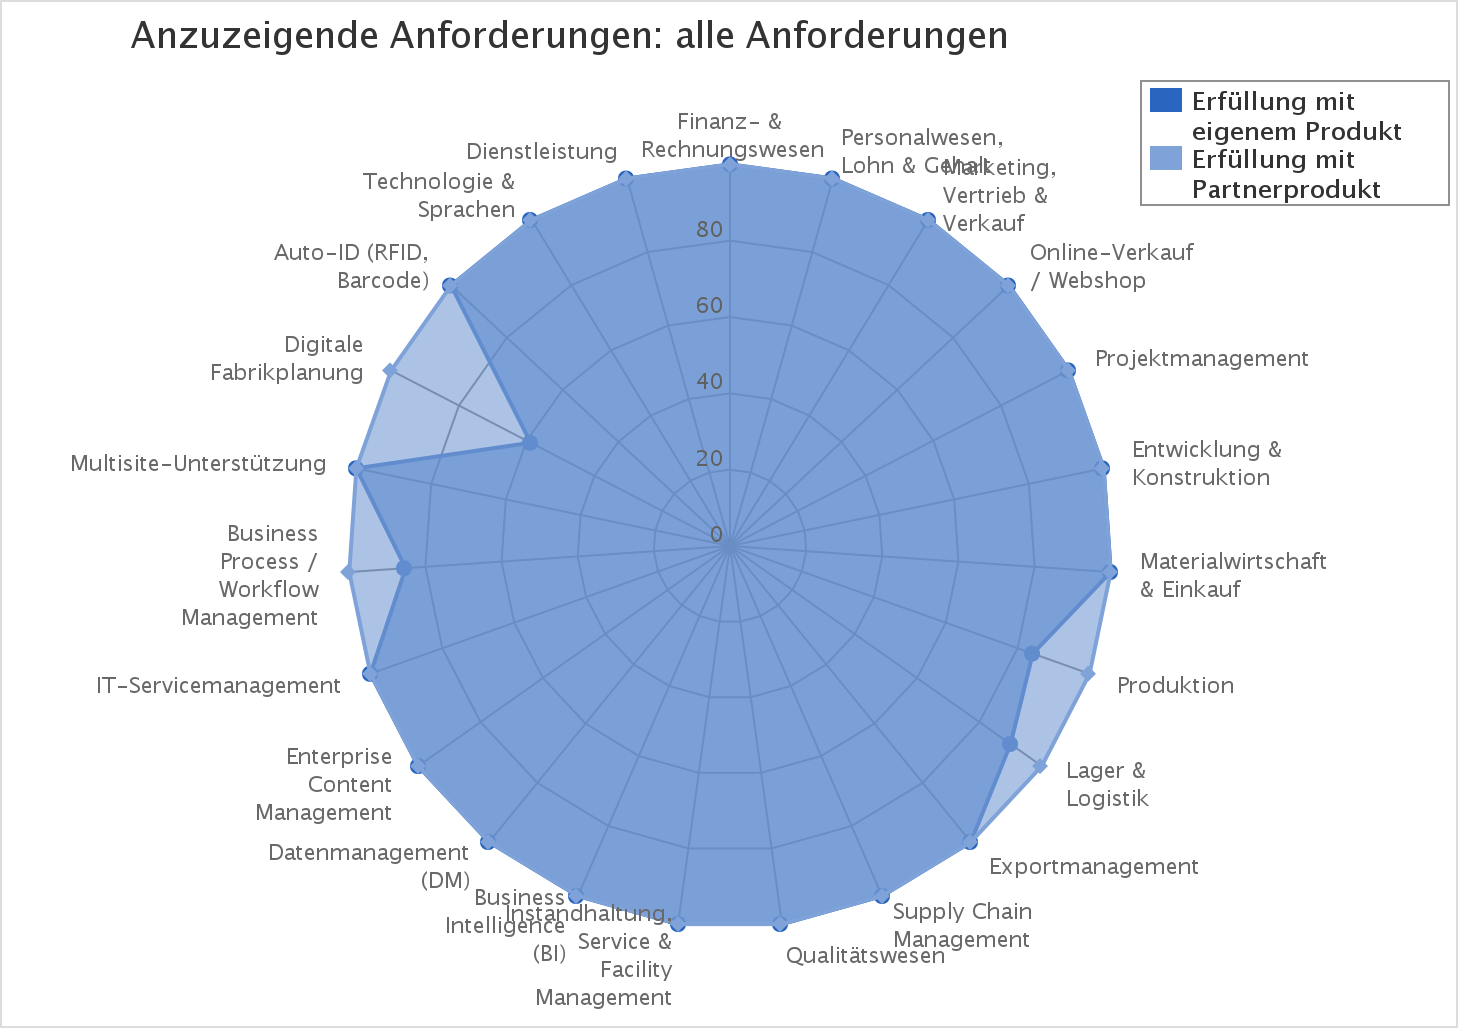
\includegraphics[width=15cm]{images/chart.png}
\caption{Spinnendiagramm}
\end{center}
\end{figure}
\noindent
Das Partnerprodukt ist vorallem für die Transport- \& Tourenplanung sowie für die Digitale Fabriksplanung (Flächenbedarfsbestimmung, Layoutgestaltung) notwendig.